\documentclass[tikz, border = 10pt]{standalone}


\usepackage{newpxtext,newpxmath}   % /upbeta
%\usepackage{fouriernc}            % /otherbeta
\usepackage{amsmath}
\renewcommand{\familydefault}{\sfdefault}
\usepackage{mathastext}

\usetikzlibrary{positioning, quotes, calc, math, arrows.meta, bending, shapes, backgrounds}

\tikzset{
every edge quotes/.style = {fill = white},
every node/.style = {scale = 1.1},
manifest/.style = {rectangle, draw, thin, inner sep = 3pt, minimum width = 1cm,
   minimum height = .85cm, align = center},
latent/.style = {ellipse, draw, thin, inner sep = 3pt, minimum width = 1cm,
   minimum height = .85cm},
residual1/.style = {circle, draw, thin, minimum size = 5mm, inner sep = 1pt},
residual2/.style = {rectangle, minimum width = 0.5pt, minimum height = 1.5mm,
   inner sep = 0pt, outer sep = 0mm},
regression/.style = {-{Stealth[length = 1.5mm]}, thin, shorten > = 1pt, 
   inner sep = 1.5pt, outer sep = 0mm},
covariance/.style={{Stealth[length = 1.5mm]}-{Stealth[length = 1.5mm]}, thin,
   shorten > = 1pt, shorten < = 1pt, inner sep = 1.5pt},
variance/.style={{Stealth[length = 1mm]}-{Stealth[length = 1mm]}, thin,
   shorten > = 1pt, shorten < = 1pt, inner sep = 1pt},
interaction/.style = {-{Stealth[sep = 1pt, length = 1.5mm] . Circle[length = 4pt]},
   thin, shorten > = -2pt},
constant/.style = {draw, thin, inner sep = 1pt, regular polygon,
   regular polygon sides = 3, minimum size = 5mm},
group/.style = {rectangle, inner sep = 2pt, minimum width = 15mm, minimum height = 5mm, 
   align = center}
}

\begin{document}
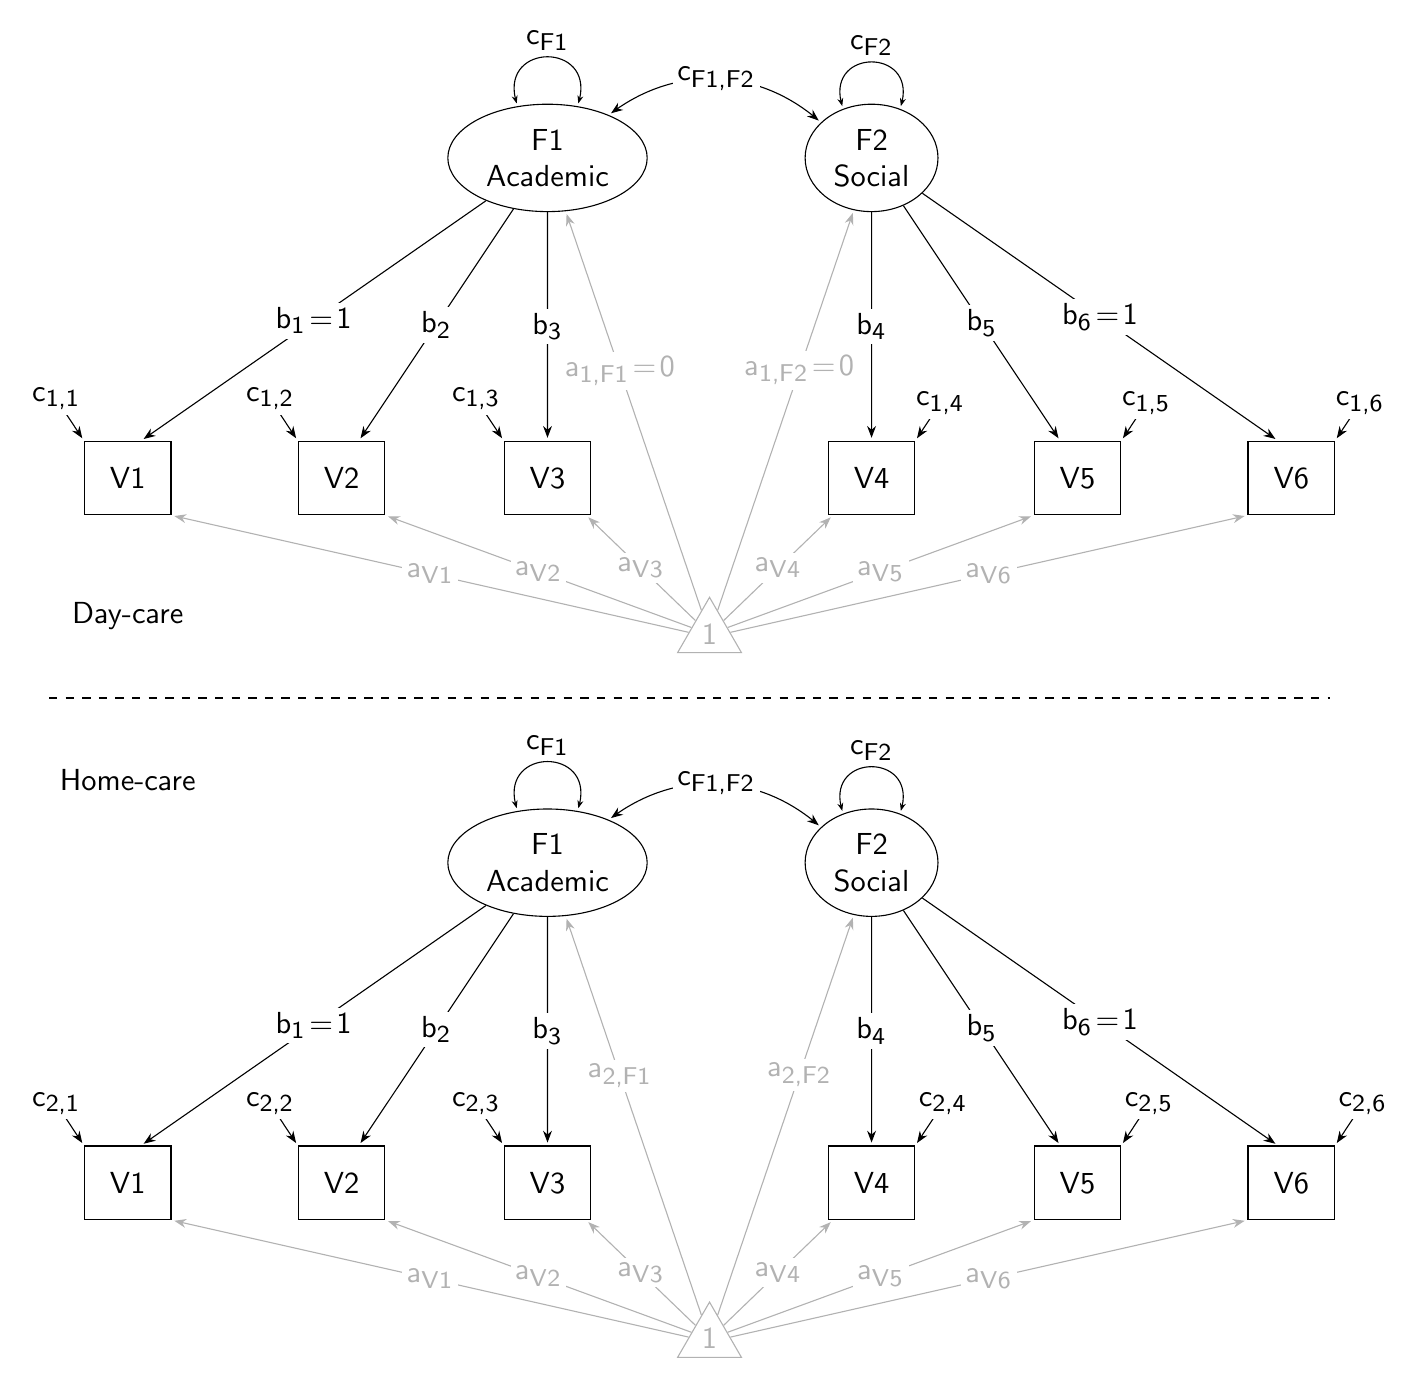
\begin{tikzpicture}

%%%% Day-care
%% Academic manifest
\node [manifest] (V11) {V1};
\node [manifest] (V12) [right = 1.6cm of V11] {V2};
\node [manifest] (V13) [right = 1.5cm of V12] {V3};

%% Social manifest
\node [manifest] (V14) [right = 3cm of V13] {V4};
\node [manifest] (V15) [right = 1.5cm of V14] {V5};
\node [manifest] (V16) [right = 1.6cm of V15] {V6};

%% Academic and Social latents
\node [latent, align = center] (F11) [above = 2.9cm of V13] {F1\\Academic};
\node [latent, align = center] (F12) [above = 2.9cm of V14] {F2\\Social};

%% Loadings
\path [regression] (F11) edge ["b$_1\!=\!1$"] (V11.70);
\path [regression] (F11) edge ["b$_2$"] (V12.65);
\path [regression] (F11) edge ["b$_3$"] (V13.90);

\path [regression] (F12) edge ["b$_4$"] (V14.90);
\path [regression] (F12) edge ["b$_5$"] (V15.115);
\path [regression] (F12) edge ["b$_6\!=\!1$"] (V16.110);

%% Latent variances ans covariance
\path [covariance] (F11.35) edge ["c$_{F1,F2}$", bend left = 40] (F12.145);
\path [variance] (F11.120) edge ["c$_{F1}$", above, outer sep = 1pt,
   bend left = 110, looseness = 3] (F11.60);
\path [variance] (F12.120) edge ["c$_{F2}$", above, outer sep = 1pt,
   bend left = 110, looseness = 3] (F12.60);

%% Residuals
\node [residual2] (e71) [above left = .65cm of V11, xshift = 1mm] {};
\path [regression] (e71) edge ["c$_{1,1}$", pos = 0] (V11.north west);

\node [residual2] (e72) [above left = .65cm of V12, xshift = 1mm] {};
\path [regression] (e72) edge ["c$_{1,2}$", pos = 0] (V12.north west);

\node [residual2] (e73) [above left = .65cm of V13, xshift = 1mm] {};
\path [regression] (e73) edge ["c$_{1,3}$", pos = 0] (V13.north west);

\node [residual2] (e74) [above right = .65cm of V14, xshift = -1mm] {};
\path [regression] (e74) edge ["c$_{1,4}$", pos = 0.1] (V14.north east);

\node [residual2] (e75) [above right = .65cm of V15, xshift = -1mm] {};
\path [regression] (e75) edge ["c$_{1,5}$", pos = 0.1] (V15.north east);

\node [residual2] (e76) [above right = .65cm of V16, xshift = -1mm] {};
\path [regression] (e76) edge ["c$_{1,6}$", pos = 0.1] (V16.north east);

%% Latent means
\node [constant, black!30] (M7) [below = 1.5cm of $(V13)!0.5!(V14)$] {1};
\path [regression, black!30] (M7) edge ["a$_{1,F1}\!=\!0$", pos = .6] (F11);
\path [regression, black!30] (M7) edge ["a$_{1,F2}\!=\!0$", pos = .6] (F12);

%% Intercepts
\path [regression, black!30] (M7.175) edge ["a$_{V1}$"] (V11.south east);
\path [regression, black!30] (M7) edge ["a$_{V2}$"] (V12.south east);
\path [regression, black!30] (M7) edge ["a$_{V3}$"] (V13);

\path [regression, black!30] (M7) edge ["a$_{V4}$"] (V14);
\path [regression, black!30] (M7) edge ["a$_{V5}$"] (V15.south west);
\path [regression, black!30] (M7.5) edge ["a$_{V6}$"] (V16.south west);

%%%% Home-care
%% Academic manifest
\node [manifest] (V21) [below = 8.0cm of V11] {V1};
\node [manifest] (V22) [right = 1.6cm of V21] {V2};
\node [manifest] (V23) [right = 1.5cm of V22] {V3};

%% Social manifest
\node [manifest] (V24) [right = 3cm of V23] {V4};
\node [manifest] (V25) [right = 1.5cm of V24] {V5};
\node [manifest] (V26) [right = 1.6cm of V25] {V6};

%% Academic and Social latents
\node [latent, align = center] (F21) [above = 2.9cm of V23] {F1\\Academic};
\node [latent, align = center] (F22) [above = 2.9cm of V24] {F2\\Social};

%% Loadings
\path [regression] (F21) edge ["b$_1\!=\!1$"] (V21.70);
\path [regression] (F21) edge ["b$_2$"] (V22.65);
\path [regression] (F21) edge ["b$_3$"] (V23.90);

\path [regression] (F22) edge ["b$_4$"] (V24.90);
\path [regression] (F22) edge ["b$_5$"] (V25.115);
\path [regression] (F22) edge ["b$_6\!=\!1$"] (V26.110);

%% Latent variances ans covariance
\path [covariance] (F21.35) edge ["c$_{F1,F2}$", bend left = 40] (F22.145);
\path [variance] (F21.120) edge ["c$_{F1}$", above, outer sep = 1pt,
   bend left = 110, looseness = 3] (F21.60);
\path [variance] (F22.120) edge ["c$_{F2}$", above, outer sep = 1pt,
   bend left = 110, looseness = 3] (F22.60);

%% Residuals
\node [residual2] (e81) [above left = .65cm of V21, xshift = 1mm] {};
\path [regression] (e81) edge ["c$_{2,1}$", pos = 0] (V21.north west);

\node [residual2] (e82) [above left = .65cm of V22, xshift = 1mm] {};
\path [regression] (e82) edge ["c$_{2,2}$", pos = 0] (V22.north west);

\node [residual2] (e83) [above left = .65cm of V23, xshift = 1mm] {};
\path [regression] (e83) edge ["c$_{2,3}$", pos = 0] (V23.north west);

\node [residual2] (e84) [above right = .65cm of V24, xshift = -1mm] {};
\path [regression] (e84) edge ["c$_{2,4}$", pos = 0] (V24.north east);

\node [residual2] (e85) [above right = .65cm of V25, xshift = -1mm] {};
\path [regression] (e85) edge ["c$_{2,5}$", pos = 0] (V25.north east);

\node [residual2] (e86) [above right = .65cm of V26, xshift = -1mm] {};
\path [regression] (e86) edge ["c$_{2,6}$", pos = 0] (V26.north east);

%% Latent means
\node [constant, black!30] (M8) [below = 1.5cm of $(V23)!0.5!(V24)$] {1};
\path [regression, black!30] (M8) edge ["a$_{2,F1}$", pos = .6] (F21);
\path [regression, black!30] (M8) edge ["a$_{2,F2}$", pos = .6] (F22);

%% Intercepts
\path [regression, black!30] (M8.175) edge ["a$_{V1}$"] (V21.south east);
\path [regression, black!30] (M8) edge ["a$_{V2}$"] (V22.south east);
\path [regression, black!30] (M8) edge ["a$_{V3}$"] (V23);

\path [regression, black!30] (M8) edge ["a$_{V4}$"] (V24);
\path [regression, black!30] (M8) edge ["a$_{V5}$"] (V25.south west);
\path [regression, black!30] (M8.5) edge ["a$_{V6}$"] (V26.south west);

%% Groups
\node (gp1) at (0,-1.75) {Day-care};
\node (gp2) [below = 1.5cm of gp1] {Home-care};

\node (C1) at ($(gp1)!0.5!(gp2)$) {};
\node (C2) [right = 14cm of C1] {};
\draw[dashed, thick] ($(C1)!-1cm!(C2)$) -- ($(C2)!-1cm!(C1)$);

\end{tikzpicture}
\end{document}





